\chapter{Design and Development: Software }
\label{processing}

\section{Installation of Necessary Applications}
\label{installation}

This setup is based on the Raspbian Jessie. It is possible to replicate the results with similar Linux-based OS but with a few minor adjustments. It assumes the complete installation of the Raspbian Jessie on the Raspberry Pi as seen in Appendix \ref{appraspbianjessie}. 

The following programs are required for the complete functionality of the WVSMS using the Raspberry Pi Terminals running on Raspbian Jessie: 

\begin{itemize}
	\item \textbf{Tight VNC Server} - Set up VNC server required to access the Raspberry Pi with its internal programs and applications \cite{rpitightvncserver}.
	\item \textbf{X Tight VNC Viewer} - Allows the Display-connected Terminal to access and view the Sensor-connected Terminal via the VNC server	\cite{rpitightvncserver}.
	\item \textbf{Arduino} - Provides analog-to-digital interface between Sensor and Terminal, converts the signal into a serial input for processing, and visualisation \cite{arduino}.
	\item \textbf{Matplotlib} - Software which renders graphs from text files \cite{matplotlib}.
	\item \textbf{Processing 2.2.1} - Software sketchbook which receives serial inputs and renders real-time graphs of given information \cite{processing221}.
	\item \textbf{Java 7} - Allows Java-based applications to run on the Platform (specifically required for Processing 2.2.1) \cite{java7}.
\end{itemize}

The installation of the first four applications are relatively simple and can be done through running the following commands in the LXTerminal (default terminal emulator) of the Raspberry Pi with an Internet connection: 

\begin{lstlisting}
sudo apt-get update
sudo apt-get install tightvncserver
sudo apt-get install xtightvncviewer
sudo apt-get install arduino
sudo apt-get install python-matplotlib
\end{lstlisting}

It is possible to use the following command to install Processing but only for the latest release of the program. At the time of testing this code, the version of Processing installed is version 3.1.1. 

\begin{lstlisting}
curl https://processing.org/download/install-arm.sh | sudo sh
\end{lstlisting}

However, for the use of the ECG and PPG, Processing 2.2.1 is required, not version 3.1.1. The devices will not function with the newer versions of Processing, displaying "size()" errors. It is necessary to uninstall package 'libgles2-mesa' before using Processing to prevent startup errors related to the P2D and P3D renderers. 

To install Processing 2.2.1 \cite{installingprocessing}: 
\begin{enumerate}
	\item Download Processing 2.2.1 from https://processing.org/download/?processing for Linux 32 platforms. 
	\item Save processing-2.2.1-linux32.tgz (98.4 MB) to the Desktop in the Raspberry Pi.  
	\item Extract the tar file using the following command: 
	\begin{lstlisting}
tar xvzf processing-2.2.1-linux32.tgz
	\end{lstlisting}

\end{enumerate}

Processing 2.2.1 requires Java to operate but it only performs well on Oracle Java 7, not Oracle Java 8. By default the Raspbian Jessie ships with Oracle Java 8. 

To install Oracle Java 7 \cite{installingprocessing}: 

\begin{lstlisting}
sudo apt-get update
sudo apt-get install oracle-java7-jdk
sudo update-alternatives --config java
rm -rf ~/processing-2.2.1/java
ln -s /usr/lib/jvm/jdk-7-oracle-armhf ~/processing-2.2.1/java
\end{lstlisting}

The last two commands remove the x86 Java runtime and replace with Raspberry Pi armhf version. This is required due to the different processor architecture which the Raspberry Pi is built on, namely the ARM architecture. 

Should the folder name be different, the last command will not work. In that case, copy '/usr/lib/jvm/jdk-7-oracle-arm-vfp-hflt' to the 'java' subfolder in the "processing-2.2.1" folder \cite{installingprocessing}. 

It is also necessary to install the Java Simple Serial Connector (jSSC) for the serial connection to work between the port and Processing 2.2.1 \cite{installingprocessing}. The zip file can be obtained from the following link: 

\begin{lstlisting}
http://code.google.com/p/java-simple-serial-connector/downloads/detail?name=jSSC-2.6.0-Release.zip&can=2&q=
\end{lstlisting}

To install the Java Simple Serial Connector (jSSC) \cite{installingprocessing}: 
\begin{lstlisting}
unzip jSSC-2.6.0-Release.zip
mv jSSC-2.6.0-Release/jssc.jar ~/processing-2.1/modes/java/libraries/serial/library/
\end{lstlisting} 

The latter command overwrites the default jssc.jar file of Processing 2.2.1 with the 2.6.0 Release. 

\section{Wireless Transmission: Operation of VNC Client-Server System}

For this project, wireless communications between the Sensor-connected Terminal and the client requires the use of VNC as seen in Section \ref{vnc}. 

The VNC server used for this project is the Tight VNC Server \cite{rpitightvncserver}. After the installation of the program in Section \ref{installation} above, the VNC server has to be set up before the Raspberry Pi becomes externally accessible as seen in Figure \ref{rpi3vnc}. 

\begin{figure}[H]
	\centering
	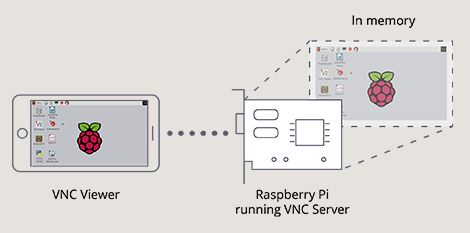
\includegraphics[width=0.7\linewidth]{rpi3vnc.jpg}
	\caption{Thermistor Formulae and Properties \cite{rpitightvncserver}}
	\label{rpi3vnc}
\end{figure}

To do this, run the following commands in LXTerminal: 

\begin{lstlisting}
sudo tightvncserver
vncserver :2 -geometry 1920x1080 -depth 24 
hostname -I
\end{lstlisting}

The first command will establish the initial settings for a VNC server and prompt for a password to authenticate and verify the user. 

The second command sets up a VNC server on the Raspberry Pi. ":2" tells the Raspberry Pi to establish the server in session 2. The resolution is set to 1920x1080 with the "-geometry" option. 

The third command reveals what IPv4 address has been allocated to the Raspberry Pi. 

The Raspberry Pi has to be connected to a WiFi network for the external connection and accessibility of its VNC server. There are two main options, namely: 

\begin{enumerate}
	\item An externally established WiFi network (through a router or gateway)
	\item An ad hoc network set up by the Raspberry Pi
\end{enumerate}

The latter choice is preferred to isolate the Raspberry Pi from a dependence on external networks. However, as a proof of concept, the former option was used for this project through a hotspot created on a local laptop with a WiFi adapter. 

Both the Sensor-connected Terminal and Display-connected Terminal must be connected on the same WiFi network. 

\subsection{Access from Another Raspberry Pi}

From the Display-connected Terminal, run Tight VNC Viewer using the following commands: 

\begin{lstlisting}
sudo xtightvncviewer
\end{lstlisting}

A prompt for the IP address and password of the VNC server will appear. After completing the details as found using the 'hostname-I' command, the graphical user interface to access the Sensor-connected Terminal will start. 

\subsection{Access from a Windows Platform}
\label{wvsmswindows}

On the Windows platform, download and install TightVNC Viewer \cite{windowstightvnc}. After completion, run TightVNC Viewer and input the IP address of the Raspberry Pi followed by the session number (':1' or ':2'). For instance: '192.168.1.2:2'. Enter the password and click 'Connect'. The graphical user interface for the Raspberry Pi will appear as in Figure \ref{vncserver}. 

\begin{figure}[H]
	\centering
	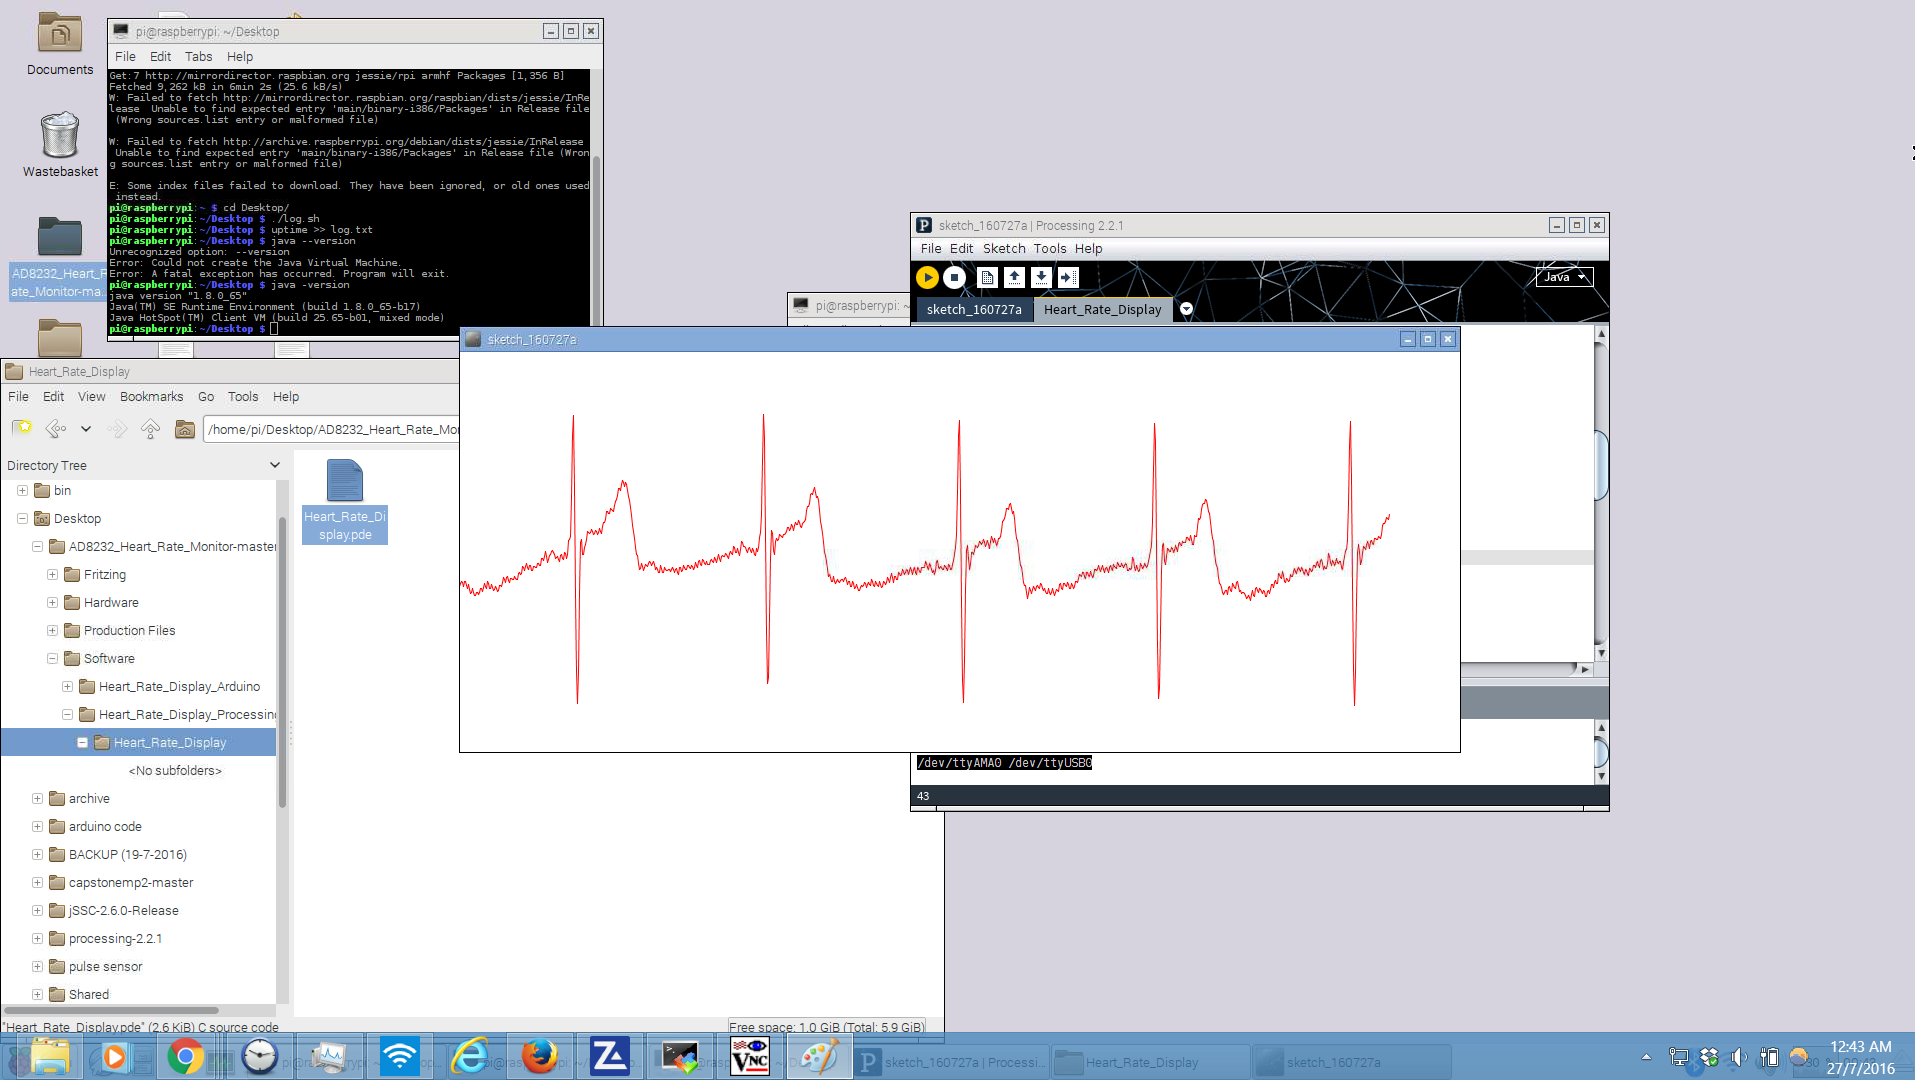
\includegraphics[width=\linewidth]{vncserver.png}
	\caption{Actual Raspberry Pi VNC Server Viewed through a VNC Viewer in a Windows Environment Wirelessly over WiFi}
	\label{vncserver}
\end{figure} 

\section{ECG Software}

The Arduino sketch from SparkFun's AD8232 Heart Rate Monitor GitHub repository must first be uploaded to the Arduino Pro Mini \cite{ad8232github} which can be found in Appendix \ref{ecgarduino}. It is important to note the board type when uploading the sketch, that is to choose Arduino Pro Mini 328 - 3.3V/8MHz. 

Next, run Processing 2.2.1 and open the pde type file from the same repository \cite{ad8232github} which can be found in Appendix \ref{ecgprocessing}. Change 'myPort = new Serial(this, Serial.list()[1], 9600);' depending on which serial port is used. 

\section{Thermistor with Phase Shift Oscillator Software}

The Arduino sketch written for the phase shift oscillator must first be uploaded to the Arduino Uno which can be found in Appendix \ref{arduinopso}.

